\setAuthor{Riho Taba}
\setRound{piirkonnavoor}
\setYear{2007}
\setNumber{G 9}
\setDifficulty{7}
\setTopic{Staatika}

\prob{Kuubik}
Kuubik massiga $m = \SI{10}{kg}$ ning küljepikkusega $a = \SI{0,1}{m}$ lebab laual. Laua ja kuubiku vaheline hõõrdetegur on $\mu = \num{0,5}$. Kas kuubikut on võimalik käega teisele küljele lükata, avaldades vaid jõudu kuni $F = \SI{40}{N}$? Eeldada, et hõõrdetegur käe ja kuubiku vahel on väga suur ehk käsi ei libise. Raskusjõu kiirendus on $g = \SI{9,8}{m/s^2}$.

\hint
Ülesande lahendamiseks tuleb küsida: (a) kas antud jõust piisab üle serva kantimiseks; (b) ega klots seejuures libisema ei hakka? Mõlema küsimuse analüüsimiseks on mugav rakendada jõumomentide tasakaalu. Lisaks on kasulik teada, et hõõrdejõu ja toereaktsiooni resultantjõu maksimaalne nurk vertikaali suhtes on $\arctan \mu$.

\solu
Ülesande lahendamine jaguneb kaheks osaks: (a) kas antud jõust piisab üle serva kantimiseks; (b) ega klots seejuures libisema ei hakka. Analüüsides oletame, et klots on juba kallutatud teatud nurga $\varphi$ ($0 \leq \varphi \leq \ang{45}$) võrra; seejuures selgub, et $\varphi = 0$ on kõige ohtlikum olukord. Alternatiiv oleks väita intuitiivselt, et ohtlikuim on olukord $\varphi = 0$ ning uurida ainult seda juhtumit;

\begin{center}
	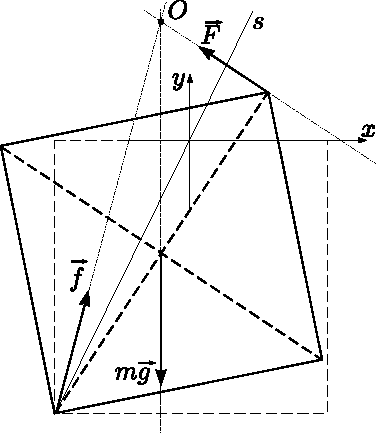
\includegraphics[height=0.6\textheight]{2007-v2g-09-lah}
\end{center}

(a) Vaatleme jõumomentide tasakaalu toetava nurga suhtes. Kompenseerimist vajab raskusjõu moment $M_{1 \mathrm{max}} = F a \cos (\ang{45}) \cos (\varphi + \ang{45})$, mille maksimaalväärtus on 
\[
M_{1 \max }=\frac{m g a}{2}, \quad M_{1 \max }=\frac{10 \cdot \num{9,8} \cdot 0,1}{2}=\SI{4,9}{N.m}.
\]
Rakendatav jõud annab seda suurema momendi, mida suurem on õlg; õla maksimaalne pikkus ei sõltu nurgast $\varphi$ ning on alati $l = a \sqrt 2$. See väärtus saavutatakse siis, kui jõud on rakendatud maha toetuva serva suhtes vastasserva külge ning on risti ruudu diagonaaliga. Seega on antud jõu abil alati võimalik tekitada raskusjõudu kompenseeriv moment väärtusega kuni
\[
M_{2}=F l=F a \sqrt{2} = \SI{5.6}{N.m}.
\]
Näeme, et $M_{1 \mathrm{max}} < M_2$, st antud jõud on piisav kuubi keeramiseks.


(b) Vaatleme jõudude tasakaalu raskusjõu $m\vec g$ ja rakendatud jõu $\vec F$ pikenduste lõikepunkti $O$ suhtes, vt joonist. Aeglasel pööramisel on jõud tasakaalus, st hõõrdejõu ja toereaktsiooni resultantjõud $\vec f$ peab minema samuti läbi selle punkti. Et hõõrdetegur $\mu = \num{0,5}$, siis nurk toetuspinna normaali (st vertikaalsihi) ja jõu $\vec f$ vahel ei tohi olla suurem, kui $\arctan \mu$, st jõud $\vec f$ ei tohi olla vähem püstine, kui sirges. Nii see ka tõepoolest on, sest punkt $O$ jääb alati piirkonda $x \leq 0$ ja $y > 0$. 

\vspace{0.5\baselineskip}

\emph{Alternatiivne lahendus osa (b) jaoks} 

Meil on vaja tõestada, et aeglasel pööramisel kehtib kogu aeg võrratus
\[
\left|F_{x}\right|=F \cos \left(\ang{45}-\varphi\right) \leq N \mu,
\]
kus $N$ on laua toereaktsioon. Paneme tähele, et vertikaalsest tasakaalutingimusest
\[
N=m g-\left|F_{y}\right|=m g-F \sin \left(\ang{45}-\varphi\right).
\]
Me kasutame osast (a) teada olevat asjaolu, et kui hõõrdumist ei oleks, siis tasakaalu tagava jõu jaoks kehtib võrratus $F < F\idx{max}$, seda asjaolu kasutame alljärgnevalt võrratuste ümber kirjutamisel.

Meile piisaks, kui suudaksime tõestada, et
\begin{equation}\label{2007-v2g-08:eq1}
\mu [mg - F\idx{max} \sin (\ang{45} - \varphi )] \geq F\idx{max} \cos (\ang{45} - \varphi ),
\end{equation}
sest sellisel juhul
\[
\begin{aligned}
N \mu &=\mu\left[m g-F \sin \left(45^{\circ}-\varphi\right)\right] \geq \mu\left[m g-F_{\max } \sin \left(\ang{45}-\varphi\right)\right] \geq \\ & \geq F_{\max } \cos \left(\ang{45}-\varphi\right) \geq F \cos \left(\ang{45}-\varphi\right)=\left|F_{x}\right|.
\end{aligned}
\]
Tõepoolest, $N\mu \geq |F_x|$. Võrratuse (\ref{2007-v2g-08:eq1}) tõestamiseks kirjutame selle ümber ekvivalentsel kujul
\[
1 \geq \frac{F_{\max }}{\mu m g}\left[\mu \sin \left(\ang{45}-\varphi\right)+\cos \left(\ang{45}-\varphi\right)\right],
\]
mis tõepoolest kehtib, sest
\[
\begin{aligned} 
& \frac{F_{\max }}{\mu m g}\left[\mu \sin \left(\ang{45}-\varphi\right)+\cos \left(45^{\circ}-\varphi\right)\right]=\\=& \frac{F_{\max } \sqrt{\mu^{2}+1}}{\mu m g} \sin \left(45^{\circ}-\varphi+\arcsin \left[\left(\mu^{2}+1\right)^{-1}\right]\right) \leq \\ \leq & \frac{F_{\max } \sqrt{\mu^{2}+1}}{\mu m g}=\frac{\SI{40}{N} \cdot \sqrt{5 / 4}}{\SI{49}{N}} \approx \num{0,91}<1. 
\end{aligned}
\]
\probend